The DOM fits on \oSixEight, \caAughtEight, \niEightFour, \snTwelveFour, and \pbEight presented in
this chapter are the culmination of the new \tot\ and \el\ experimental results
(Chapters \ref{TCSAnalysis} and \ref{ECSAnalysis})
and new computational improvements in our DOM code (Chapter \ref{DOMFormalism}).
Previous DOM treatments have either used a
local equivalent potential \cite{Charity2006, Mueller2011} that was unsuitable for extracting
negative-energy information or only provided results on one or
two nuclei \cite{Mahzoon2017}. All nine fits detailed here use the same fully-non-local approach
(outlined in chapter \ref{DOMFormalism}) and lay the groundwork for a comprehensive DOM treatment 
across the chart of nuclides.

Beginning with \caForty, the results from our new analyses of
\caAughtEight and \pbEight are compared to the previous DOM analyses of \cite{MahzoonPhDThesis} and 
\cite{Atkinson2018}. Next, results on \oSixEight, \niEightFour, and \snTwelveFour are compared to
the local treatments of \cite{Charity2006, Mueller2011}. Last, general trends are identified across
all nine nuclei and successes and deficiencies of the present DOM treatment are pointed out.
A complete list of experimental data used to constrain the fits is the subject of Appendix
\ref{DOMDataSets}. The best-fit parameter values for each nucleus are given in Appendix
\ref{DOMParameters}. Finally, complete visualizations of the experimental data used to constrain
the data, DOM predictions for these data, and structural information extracted from the DOM fits are
provided in Appendix \ref{DOMVisualization}.

\section{Results for \caAughtEight}
As doubly-closed, mid-A nuclei, \caAughtEight are heavy enough for both density functional
theory (DFT) calculations \cite{Piekarewicz2012} and light enough for \textit{ab initio} 
treatments \cite{Hagen2016}. As such, they have long been cornerstone nuclei for
nuclear modeling. The size of the neutron skin of \caEight (along with that of $^{132}$Sn and
\pbEight) is of immense theoretical interest, as it is expected to be tightly correlated with the
density-dependence of the symmetry energy \cite{Fattoyev2012}. A model-independent determination
of the neutron skin thickness of \caEight is the goal of the upcoming parity-violating
electron scattering measurement CREX \cite{CREX}. Optical models have been applied to
\caAughtEight more than almost any other nucleus. A great deal of high-quality \caAughtEight elastic 
and inelastic nucleon scattering data, quasi-free scattering data, and elastic electron
scattering data are available, making them ideal candidates to test the DOM approach. To orient the
reader and facilitate a comparison to previous DOM treatments, the \caAughtEight fit results are
presented in greater detail than are the fit results on \oSixEight, \niEightFour,
\snTwelveFour, and \pbEight presented later.

\subsection{Results for \caForty}
In keeping with previous DOM treatments of \caForty \cite{MahzoonPhDThesis}, the present fit
quickly converged on proton and neutron elastic and inelastic scattering data from 10-200
MeV (shown in Fig. \ref{CaElasticReproduced}). Because the \caForty proton \rxn\ has been
measured up to 200 MeV, the energy-dependence of the imaginary volume potential, $W_{vol}^{+}$, was
well-constrained, expediting the fitting process and lending confidence to the quality of our fit
\ref{CaReactionReproduced}. 
[comments about bound-state data fitting]
- table with spectroscopic factors of valence states
- table with particle numbers
In Figure \ref{s1Depletion}, is clear that without $\approx$30\%
depletion of the proton 1\sOne\ shell, the charge density at the core of
\caForty is too high,
a characteristic failure of mean-field models that do not account for this depletion. 

The spectral functions of \caForty nucleons that 
we extract from the fit (Fig. \ref{Ca40SpectralFunctions}) show significant occupation depletion and 
spectral peak broadening compared 
to the mean-field expectation, in keeping with (p,2p) measurements \cite{LiverpoolCa40}.

\begin{figure}[ht!]
    \centering
    \includegraphics[width=0.9\textwidth]{figures/CaElasticReproduced.png}
    \caption[Nucleon differential cross sections of \caForty: DOM predictions and experimental data]
    {
        Experimental \caForty proton and neutron differential elastic cross sections
        (panels (a) and (c)) and analyzing powers (panels (b) and (d)) are shown as points, and 
        predictions from the DOM \caForty fit of these data are shown as lines. For visibility, the 
        data have been offset along the ordinate axis so that the highest-energy data
        appear at the top of the graphs. References to all experimental data are listed
        in Appendix \ref{DOMDataSets}.
    }
    \label{CaElasticReproduced}
\end{figure}

\begin{figure}[ht!]
    \centering
    \includegraphics[width=0.9\textwidth]{figures/CaReactionReproduced.png}
    \caption[Nucleon \rxn\ of \caForty: DOM predictions and experimental data]
    {
        Experimental \caForty proton \rxn\ data (panel (a)) and neutron \tot\ and \rxn\ data (panel
        (b)) are shown as points, and 
        predictions from the DOM \caForty fit of these data are shown as lines.
        References to all experimental data are listed in Appendix \ref{DOMDataSets}.
    }
    \label{CaReactionReproduced}
\end{figure}

\begin{figure}[ht!]
    \centering
    \includegraphics[width=0.9\textwidth]{figures/Ca40SpectralFunctions.png}
    \caption[Spectral peak broadening in \caForty: DOM prediction and experimental (p,2p) data]
    {
        Spectral peak broadening is observed in nucleon knock-out experiments, a 
        consequence of increased imaginary strength in the self-energy at energies far from the
        Fermi energy. Panel (b) shows the hole spectral functions for protons in \caForty
        with orbital angular momentum $L$ and total angular momentum $J$ as predicted by our DOM fit.
        The peak location and general shape of the hole spectral functions we recover match those
        extracted from analysis of experimental (p,2p) data of \cite{LiverpoolCa40}.
    }
    \label{s1Depletion}
\end{figure}

\begin{figure}[ht!]
    \centering
    \includegraphics[width=0.9\textwidth]{figures/s1Depletion.png}
    \caption[Depletion of proton \sOne\ in \caForty essential to reproduce charge density
    distribution]
    {
        The depletion of the proton \sOne\ in \caForty is essential
        for reproducing the charge density
        distribution as calculated from experimental elastic electron scattering \cite{DeVries}.
    }
    \label{s1Depletion}
\end{figure}

From the hole spectral functions, the momentum-space distribution for protons and neutrons was
calculated (shown in Fig. \ref{Ca40Momenta}). The amount of ``high-
momentum content'' in these distributions is of great interest, as significant high-momentum content 
indicates deviation from the mean-field picture due to short-range correlations (SRCs). SRCs arise 
even in very light nuclear systems (e.g., $^{4}He$)
and appear to be responsible for the so-called EMC Effect \cite{PRC_85_047301_OHen, 
PRC_86_065204_Arrington, CLAS2019}.
Tensor-force 
interactions in neutron-proton pairs are thought to be the dominant source of 
SRCs \cite{Subedi2008}. Accordingly, in symmetric nuclei like \cTwelve and \caForty, the
high-momentum content is expected to be nearly the same for protons and neutrons, whereas in
asymmetric nuclei like \pbEight, the minority nucleon species is expected to have a larger
high-momentum tail in the momentum distribution. In \cite{C12HighMomentum}, the \cTwelve proton and
neutron momentum distributions showed that ~10\% of the total nucleon density lies above 270 MeV/c.
From our DOM fits, we calculate values of [insert ca40 momentum for p/insert ca40 momentum for n]\%
for protons and neutrons respectively, in line with the expectation that the high-momentum content
should increase slightly as one moves to higher A.

The binding energy for \caForty is readily calculated using Eq.
\ref{TotalEnergyEquation}. Its radial dependence is shown in Fig. \ref{Ca40Energies} and the
contributions to the binding energy from each single-particle LJ are shown in
\ref{Ca40EnergiesByLJ}. Per our fit, even though the 0\sOne nucleons consitute only [insert \%
of 0\sOne occupation] of the 40 nucleons in \caForty, they provide the lion's share of the binding
energy ([insert binding energy \% for protons and neutrons]). The spectral
functions make things clear: 0\sOne nucleons spend a small but significant portion of their time 
at very negative energies ($<$-100 MeV), pulling the weighted average binding energy toward
[insert Ca40 binding energy] MeV/A, the experimentally-known binding energy for \caForty. In this
picture, it is clear why mean-field models consistently underpredict the binding energy, as they
cannot adequately represent the nucleon-nucleon correlations associated with the long
negative-energy tail of the spectral functions.

Lastly, from the proton and neutron point distributions generated by our fit, we calculate a
\caForty neutron skin for of [insert neutron skin] fermi (see Fig. \ref{Ca40MatterDistributions}). 
This is in excellent agreement with the skin calculated in previous DOM treatments
\cite{MahzoonPhDThesis} and with the expectation that the neutron skin should be slightly negative in
symmetric nuclei, a consequence of Coulomb repulsion nudging proton density toward the surface.

\subsection{Results for \caEight}


\section{Results for \oSixEight}
As the lightest system analyzed in the DOM framework, \oSix is a useful test case
for the validity of the DOM in light systems and useful benchmark for $\chi$-EFT, shell model, ab
initio approaches, and other theoretical treatments. In addition, a wealth of scattering and
bound-state information have been collected on this nucleus that expose the strengths and
weaknesses of the DOM potential forms.

The experimental data used to constrain the \oSix potential and structural information extracted
from the fit are available in \ref{tab:O16ExpData} and \ref{O16DOMOutput}. Good agreement with all 
experimental data was achieved, excepting the following regimes:

- neutron total cross section at <10 MeV
- proton differential elastic cross sections and analyzing powers above 150 MeV at backward angles

For a system as light as \oSix, the density of states at low energies (i.e., below the neutron
separation energy) is sufficiently low that a smoothly-varying potential will be a poor
approximation of the resonance structure that dictates the strength of inelastic scattering. Hence,
our fit of the neutron total cross section in \oSix fails to reproduce the resonance structures and
instead generates an average behavior over these resonances.

Of the nuclides we chose for a DOM treatment, \oEight was the most difficult due to the paucity of
available experimental data, the lightness of the system, and the neutron open shell. To constrain the negative-energy domain
of the potential, the only available experimental data were the neutron and proton separation
energies and the RMS charge radius of \oEight and \neEight. Accordingly, the uncertainty in our extracted structural quantities is
larger than in any other system we studied.

Because no \oEight charge density distribution was available, we generated an approximate charge density
distribution for \oEight by linearly scaling
the radii and densities of the \oSix charge density distribution to reproduce the \oEight RMS charge
radius and maintain a total charge of 8. The reported RMS charge radii of \oSix and \oEight differ by only
0.01 fm (<0.5\%), so the approximate \oEight charge density distribution we generated is barely
distinguishable from the \oSix distribution. This same scaling procedure was also employed to
generate a charge density distribution for \snTwelve, using the
experimentally-derived \snFour charge density distribution. To initiate the fit, the \oSix best-fit parameter values
were assigned to the \oEight parameter file and calculated observables were generated to compare
with \oEight data. Unsurprisingly, the \oSix parameter values were moderately successful at reproducing
the \oEight scattering data without further adjustment, though almost no neutron scattering data is
available besides our newly-measured \tot. Using the \oSix parameters, the \oEight valence SP levels were underbound
by several MeV and the recovered particle number was too low, clearly a result of the insufficient
depth of the \oSix HF term compared to that required for additional binding in \oEight. Thus, before
loosening any other parameters, the HF depth and HF depth asymmetry terms were allowed to vary,
reducing the chi-square contribution from the charge density, particle number, and energy level
sectors. Once a chi-square minimum had been reached with these two parameters, all other symmetric parameters
were allowed to vary.

%\begin{figure}
%\begin{center}
%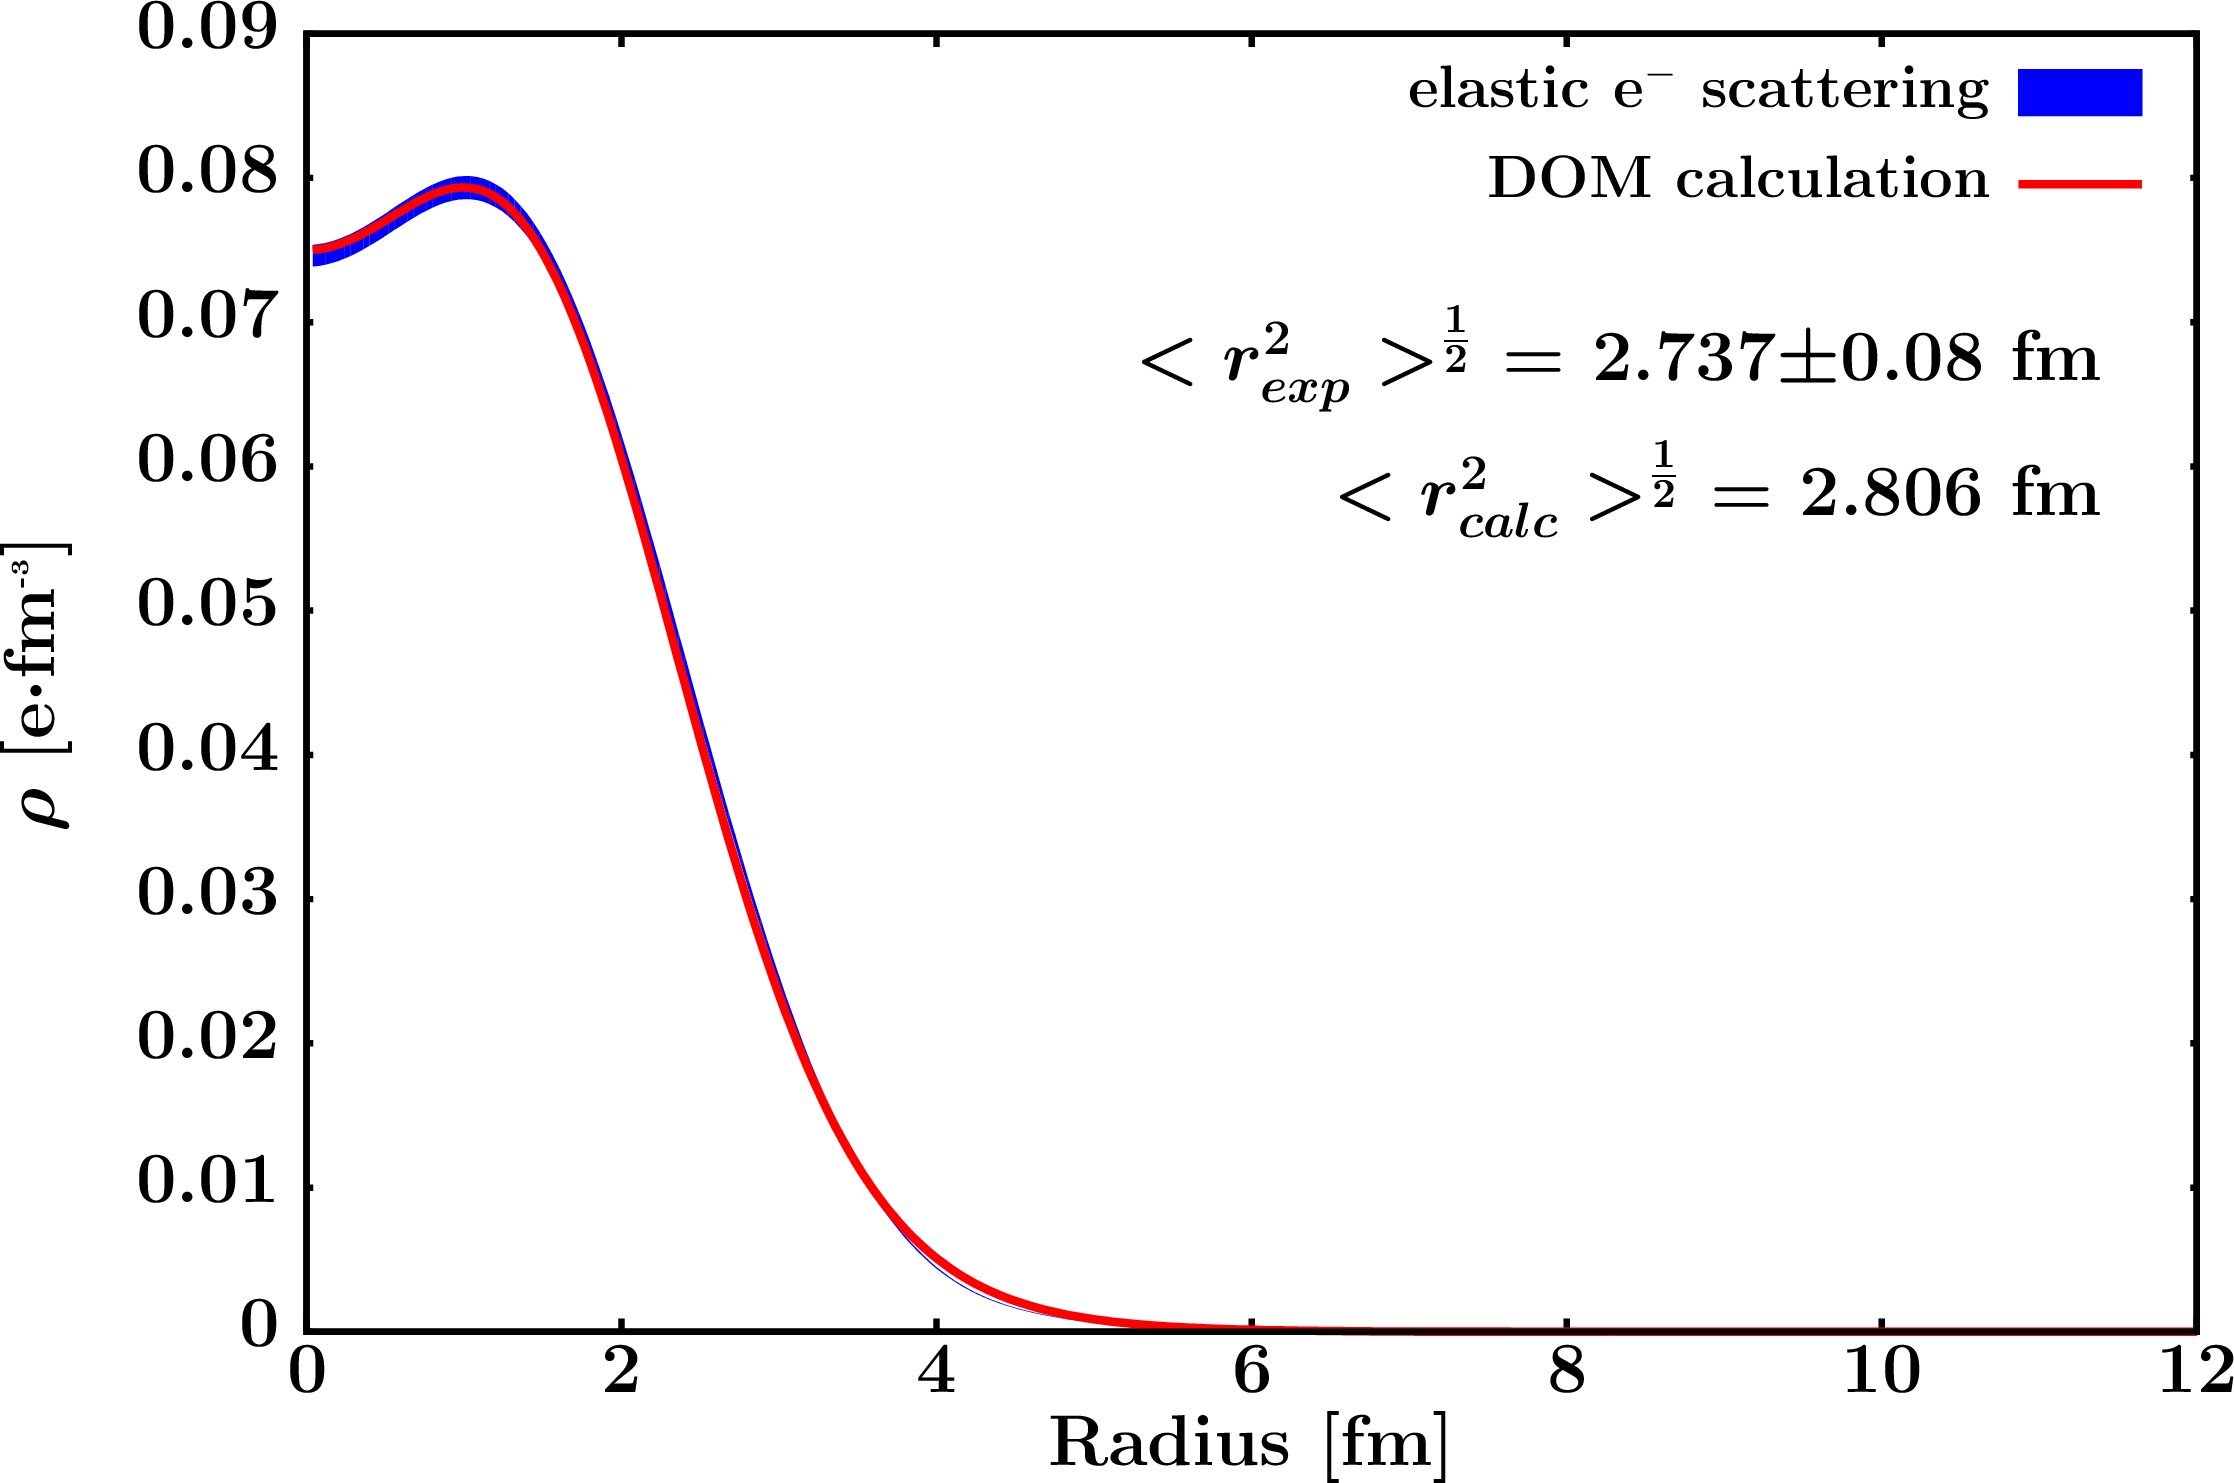
\includegraphics[width = 0.9\textwidth]{figures/o16_chargeDensity.png}
%\caption{DOM fit of  charge density}
%\label{o16ChargeDensity}
%\end{center}
%\end{figure}
%
%\begin{figure}
%\begin{center}
%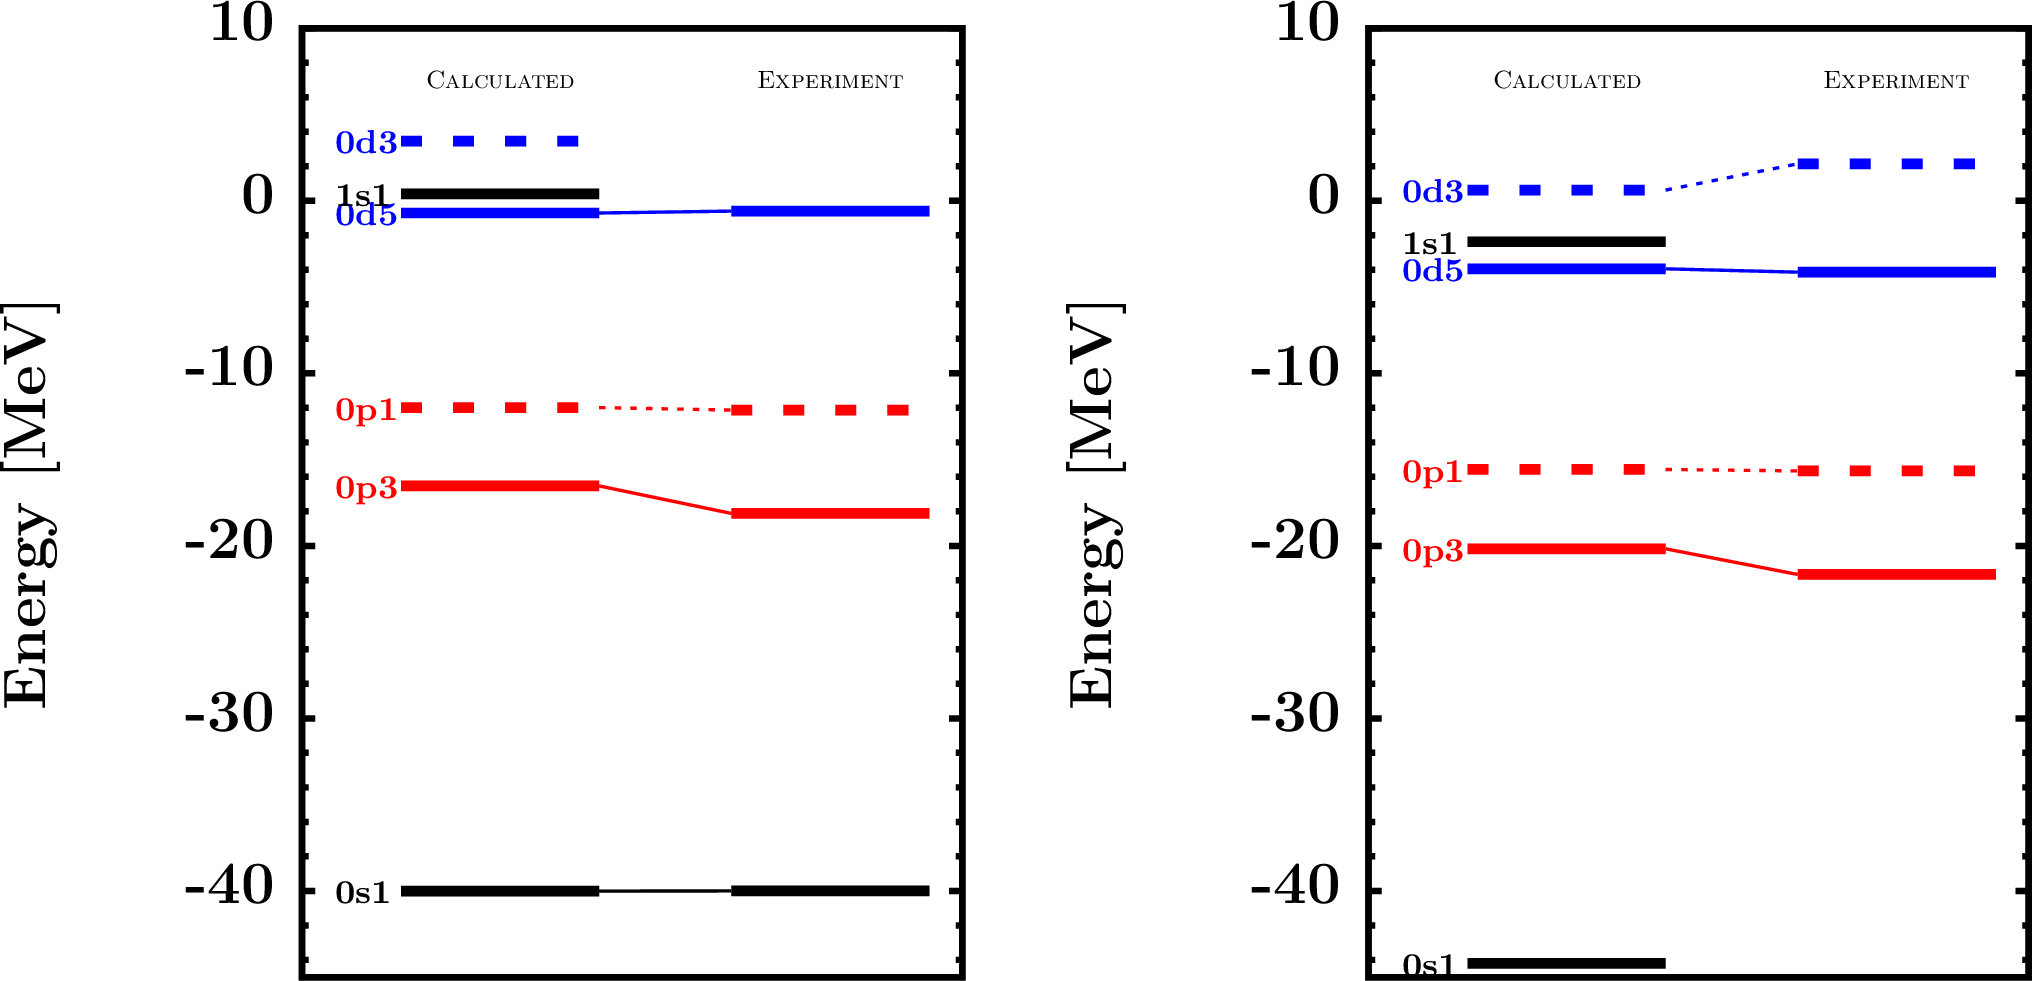
\includegraphics[width = 0.9\textwidth]{figures/o16_SPLevels.png}
%\caption{DOM fit of $^{16}O$ single-particle levels}
%\label{o16SPLevels}
%\end{center}
%\end{figure}
%
%\begin{figure}
%\begin{center}
%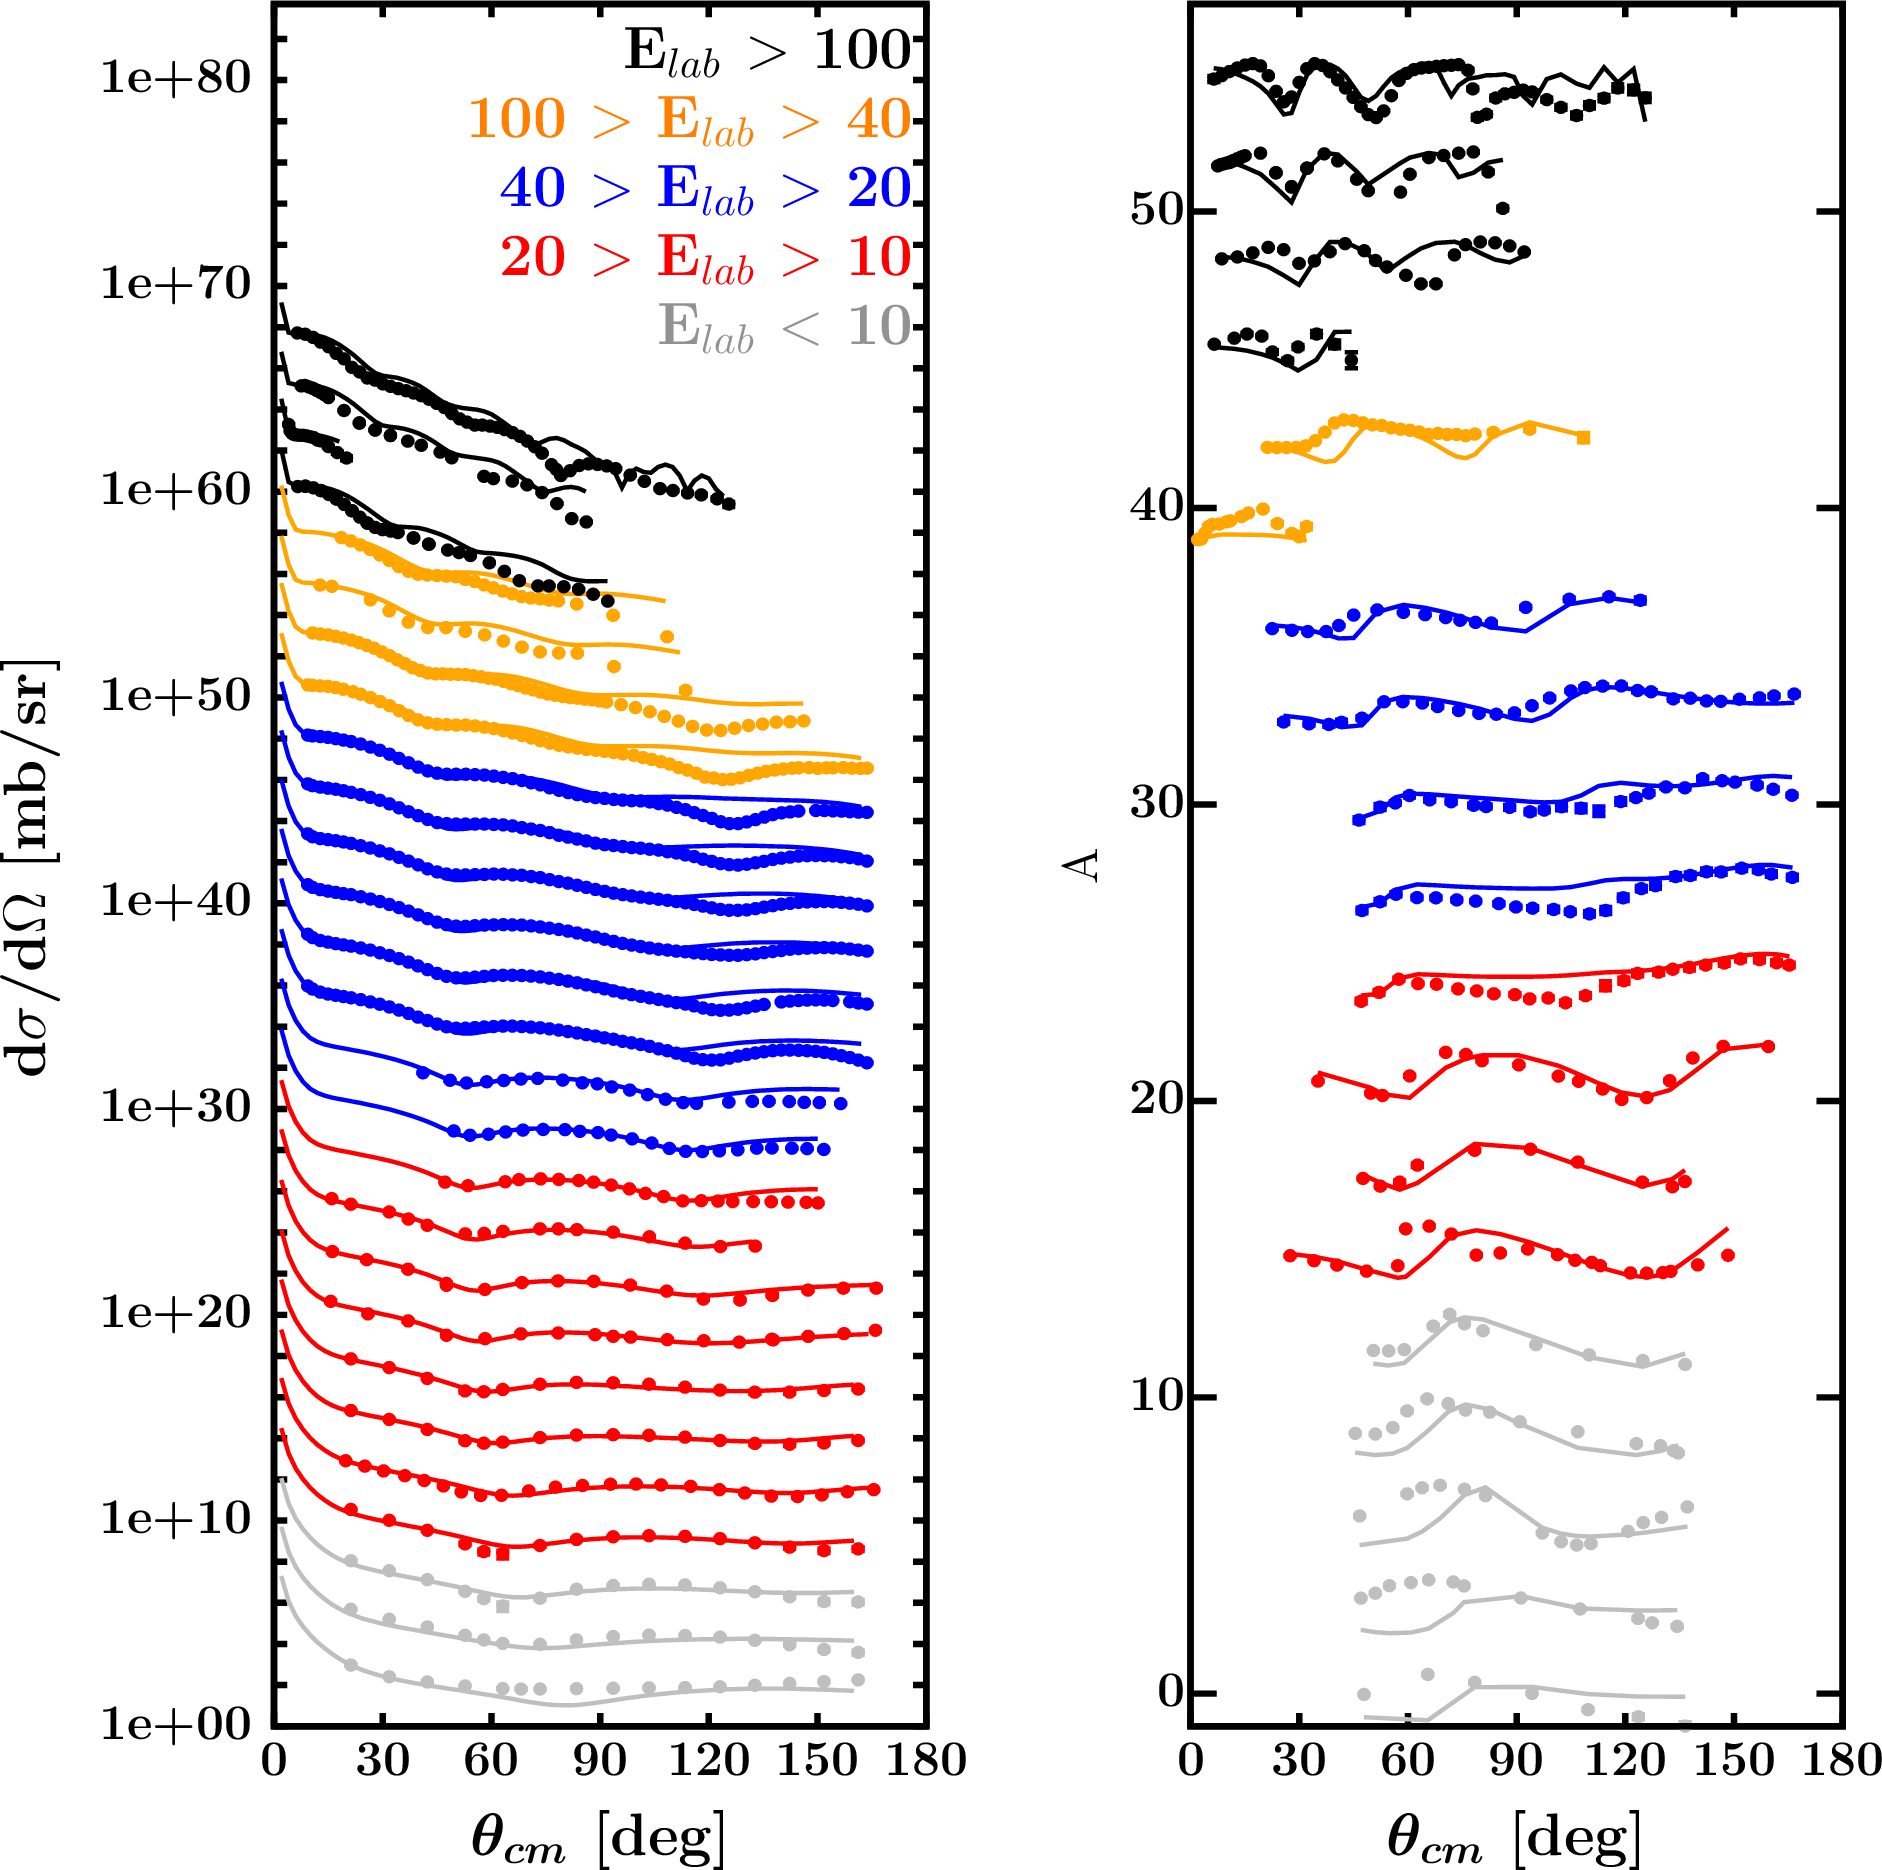
\includegraphics[width = 0.9\textwidth]{figures/o16_protonElastic.png}
%\caption{DOM fit of $^{16}O$ proton elastic scattering data}
%\label{o16ProtonElastic}
%\end{center}
%\end{figure}
%
%\begin{figure}
%\begin{center}
%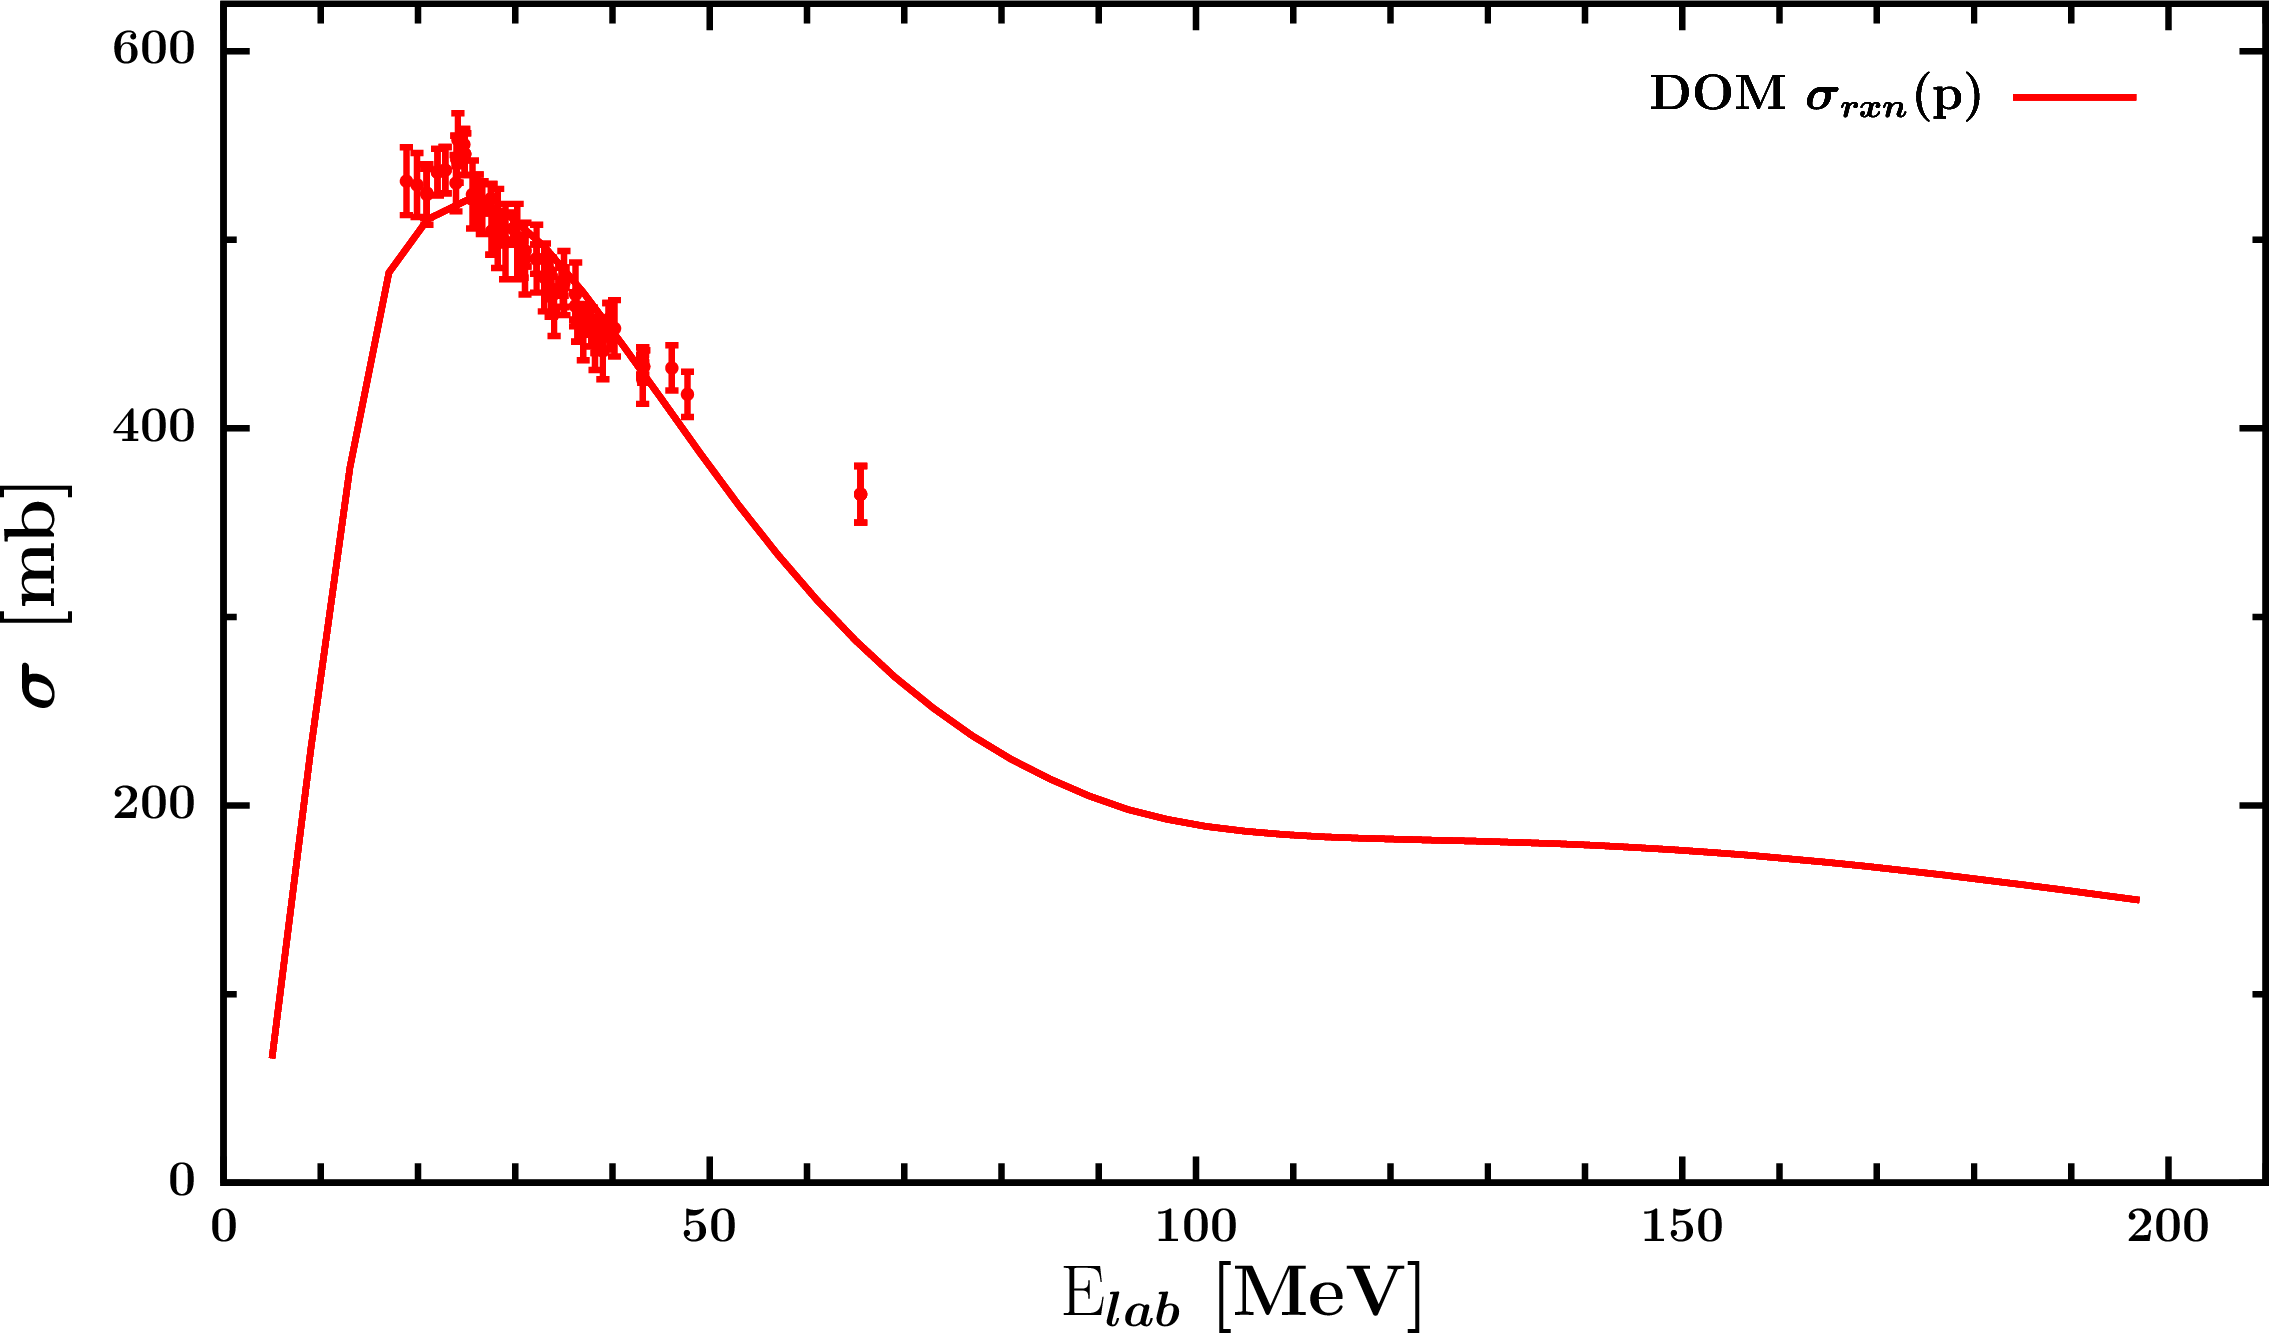
\includegraphics[width = 0.9\textwidth]{figures/o16_protonInelastic.png}
%\caption{DOM fit of $^{16}O$ proton inelastic scattering data}
%\label{o16ProtonInelastic}
%\end{center}
%\end{figure}
%
%\begin{figure}
%\begin{center}
%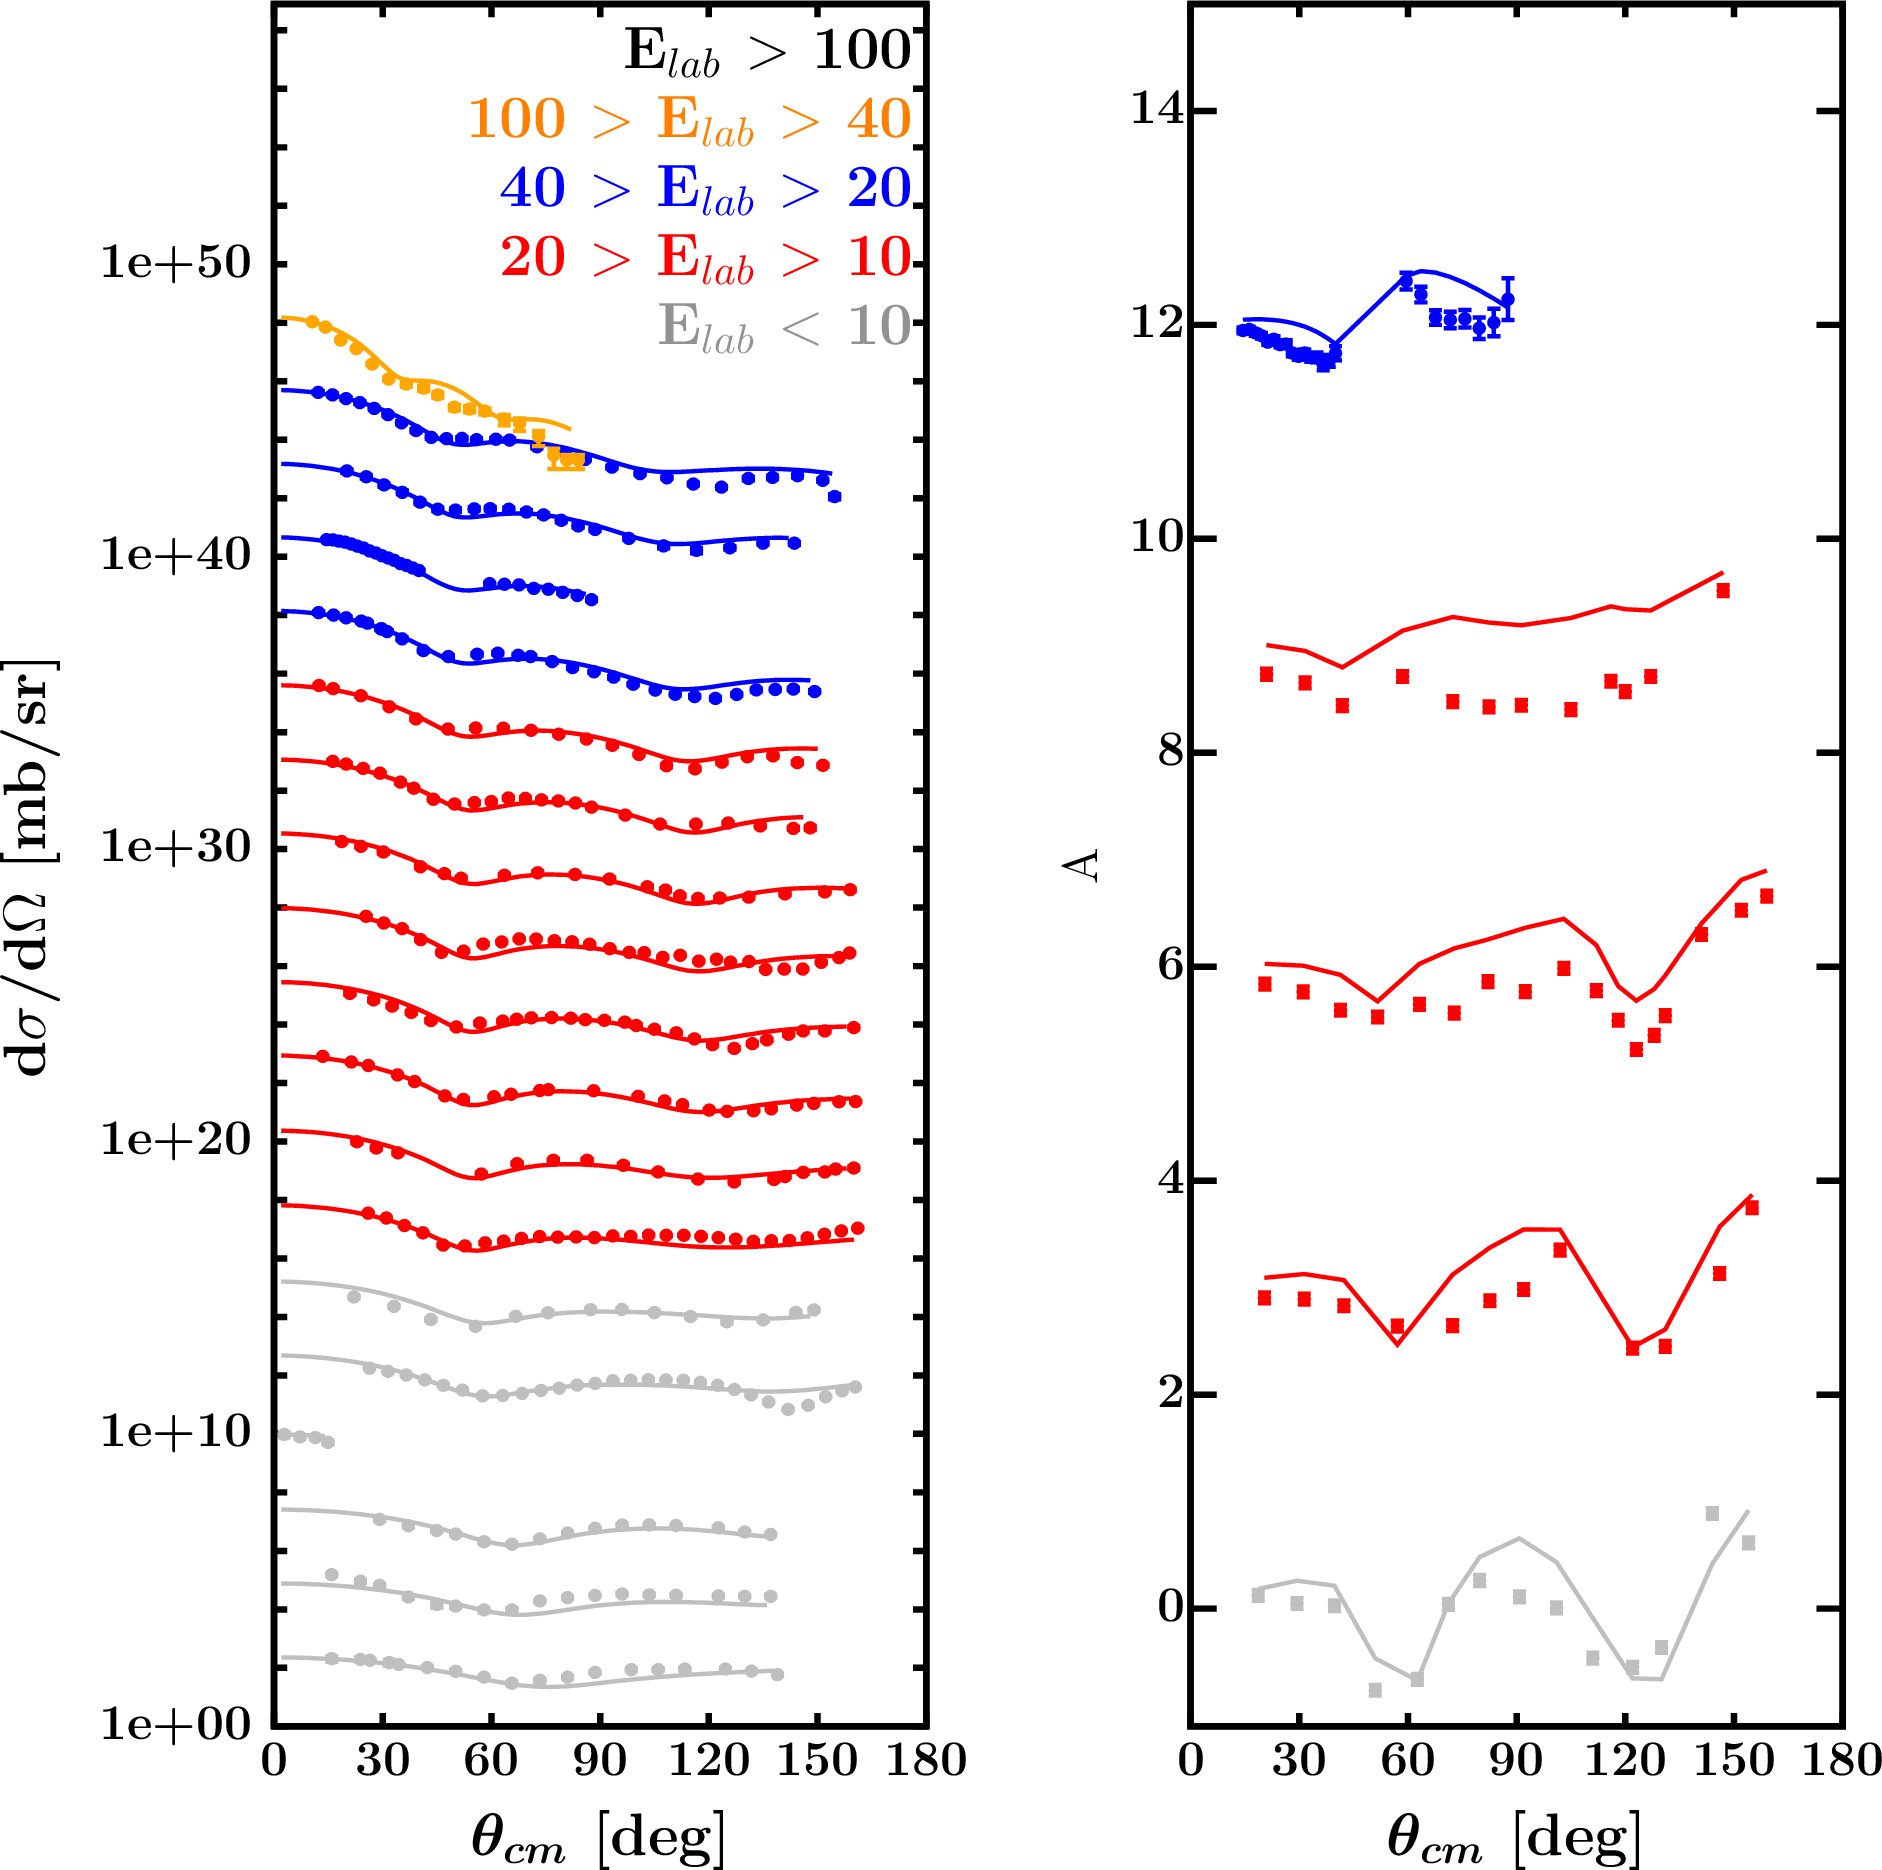
\includegraphics[width = 0.9\textwidth]{figures/o16_neutronElastic.png}
%\caption{DOM fit of $^{16}O$ neutron elastic scattering data}
%\label{o16NeutronElastic}
%\end{center}
%\end{figure}
%
%\begin{figure}
%\begin{center}
%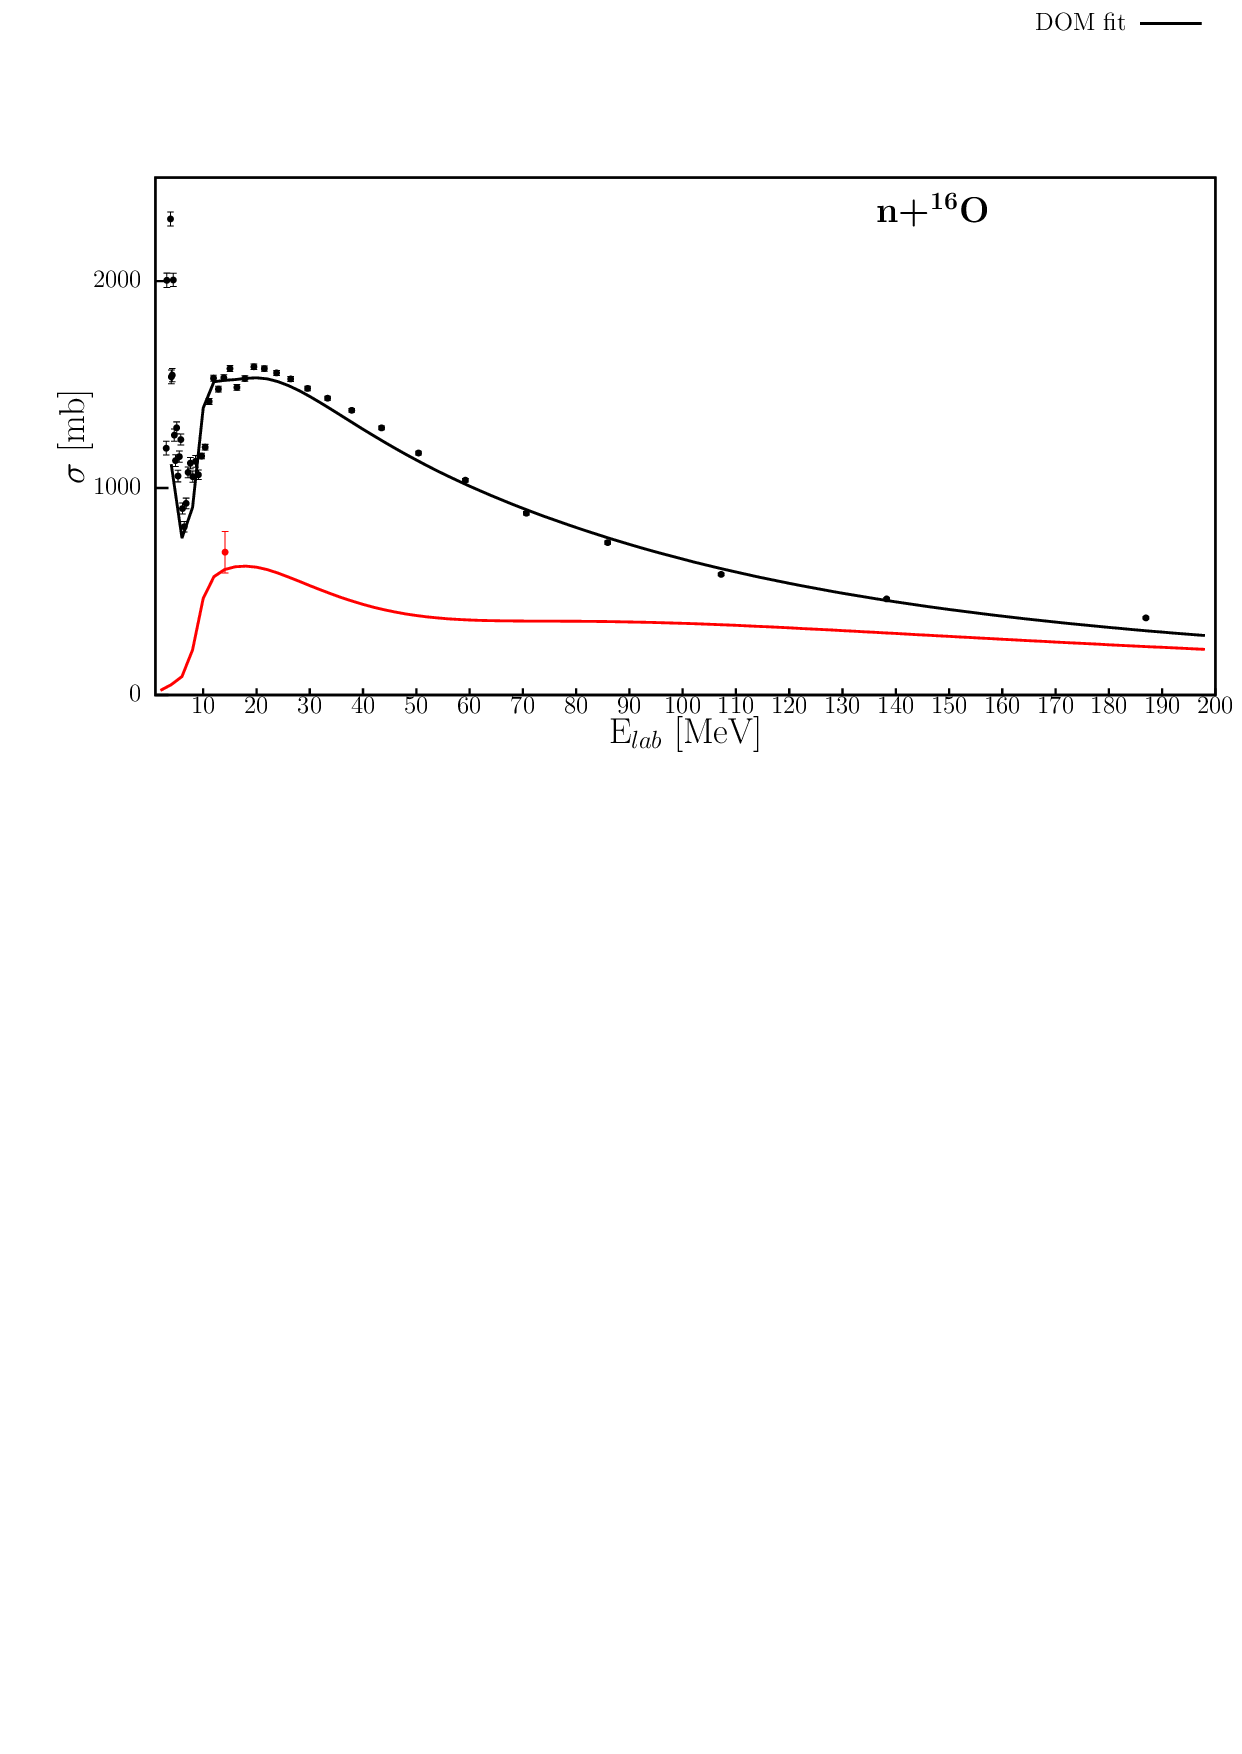
\includegraphics[width = 0.9\textwidth]{figures/o16_neutronInelastic.png}
%\caption{DOM fit of $^{16}O$ neutron inelastic scattering data}
%\label{o16NeutronInelastic}
%\end{center}
%\end{figure}
%
%\begin{figure}
%\begin{center}
%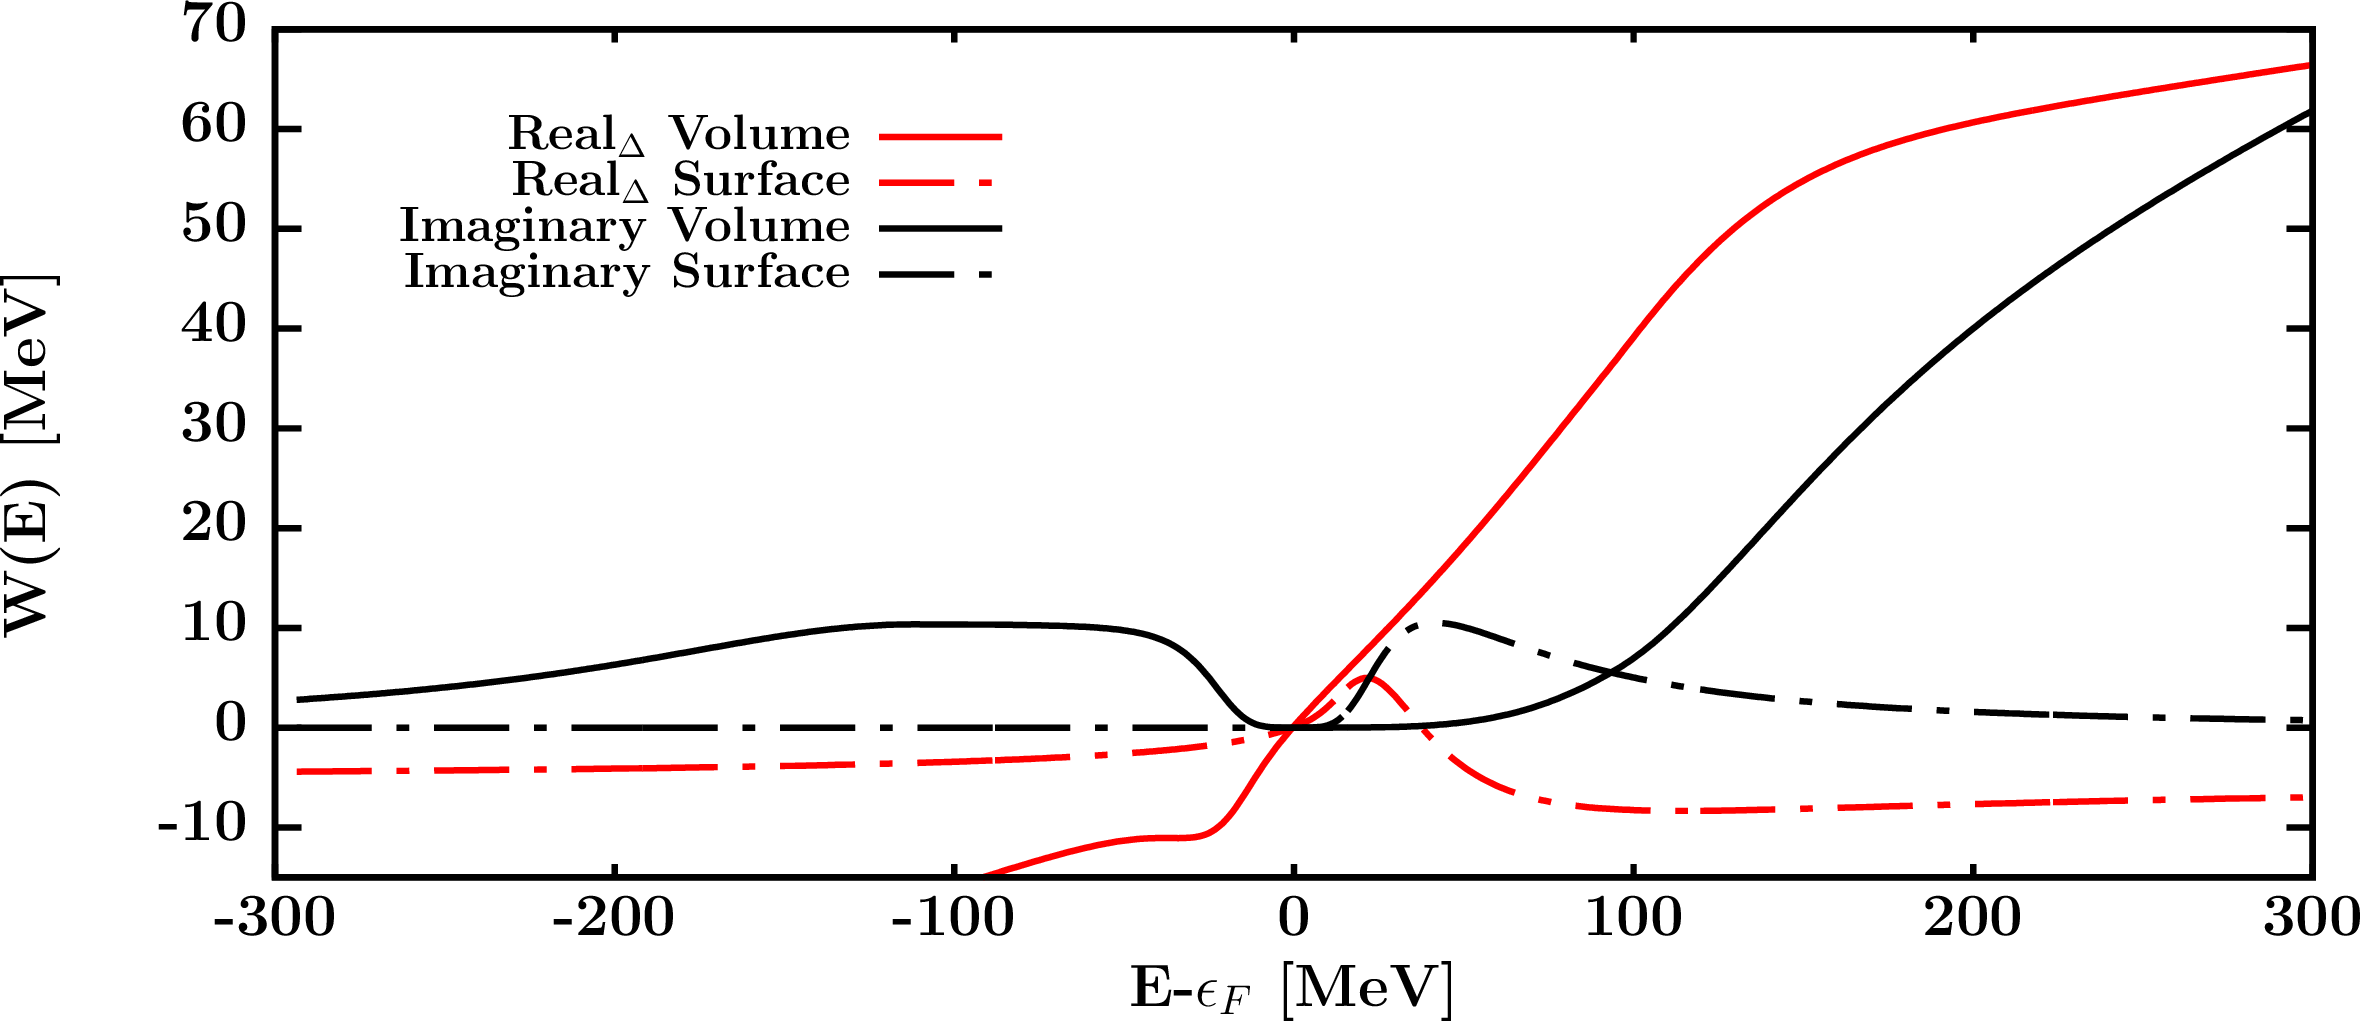
\includegraphics[width = 0.9\textwidth]{figures/o16_protonPotentials.png}
%\caption{Visualization of DOM optical potential components for protons on
%$^{16}O$}
%\label{o16ProtonPotentials}
%\end{center}
%\end{figure}
%
%\begin{figure}
%\begin{center}
%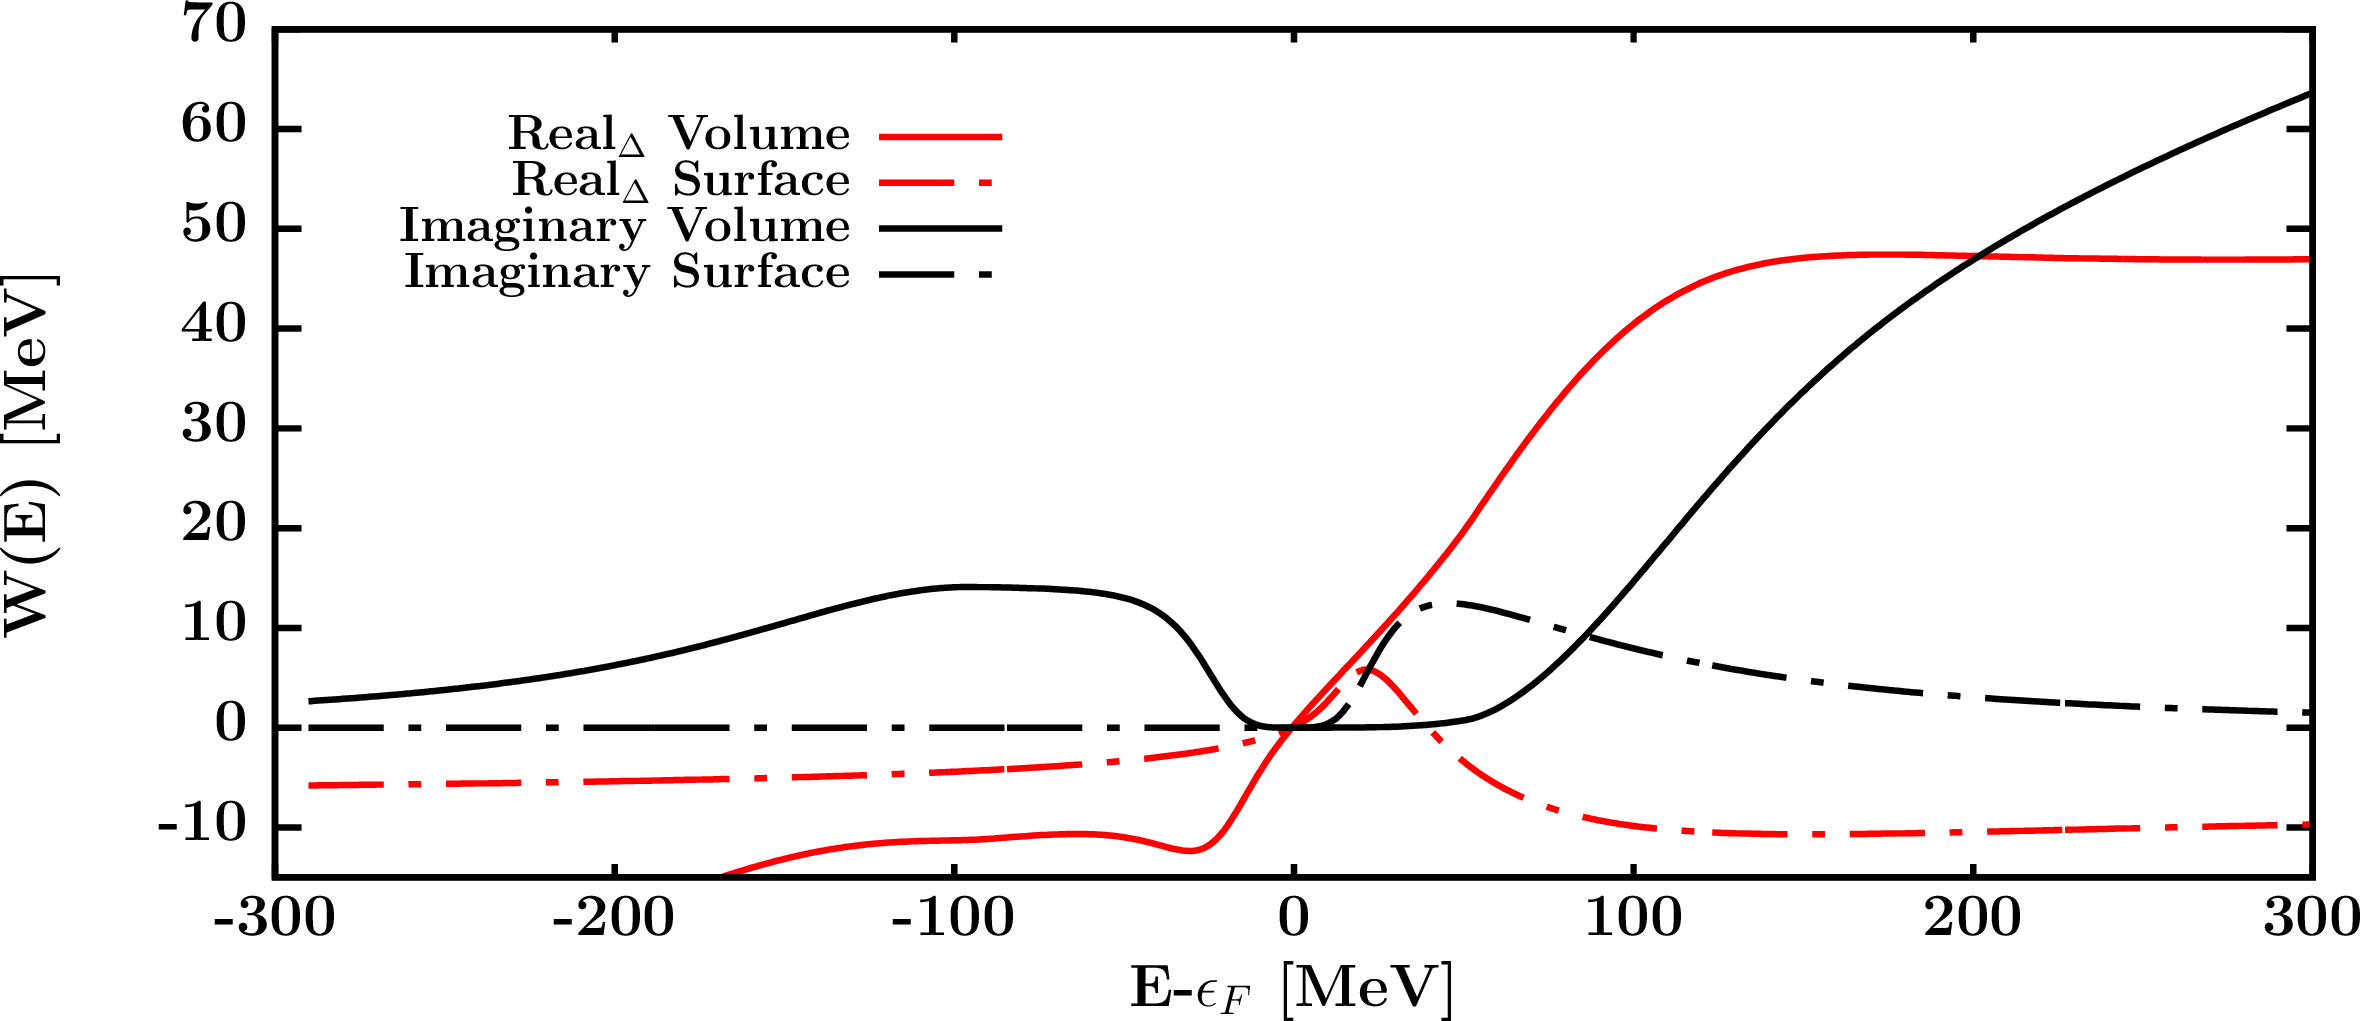
\includegraphics[width = 0.9\textwidth]{figures/o16_neutronPotentials.png}
%\caption{Visualization of DOM optical potential components for neutrons on
%$^{16}O$}
%\label{o16NeutronPotentials}
%\end{center}
%\end{figure}
%
%\begin{figure}
%\begin{center}
%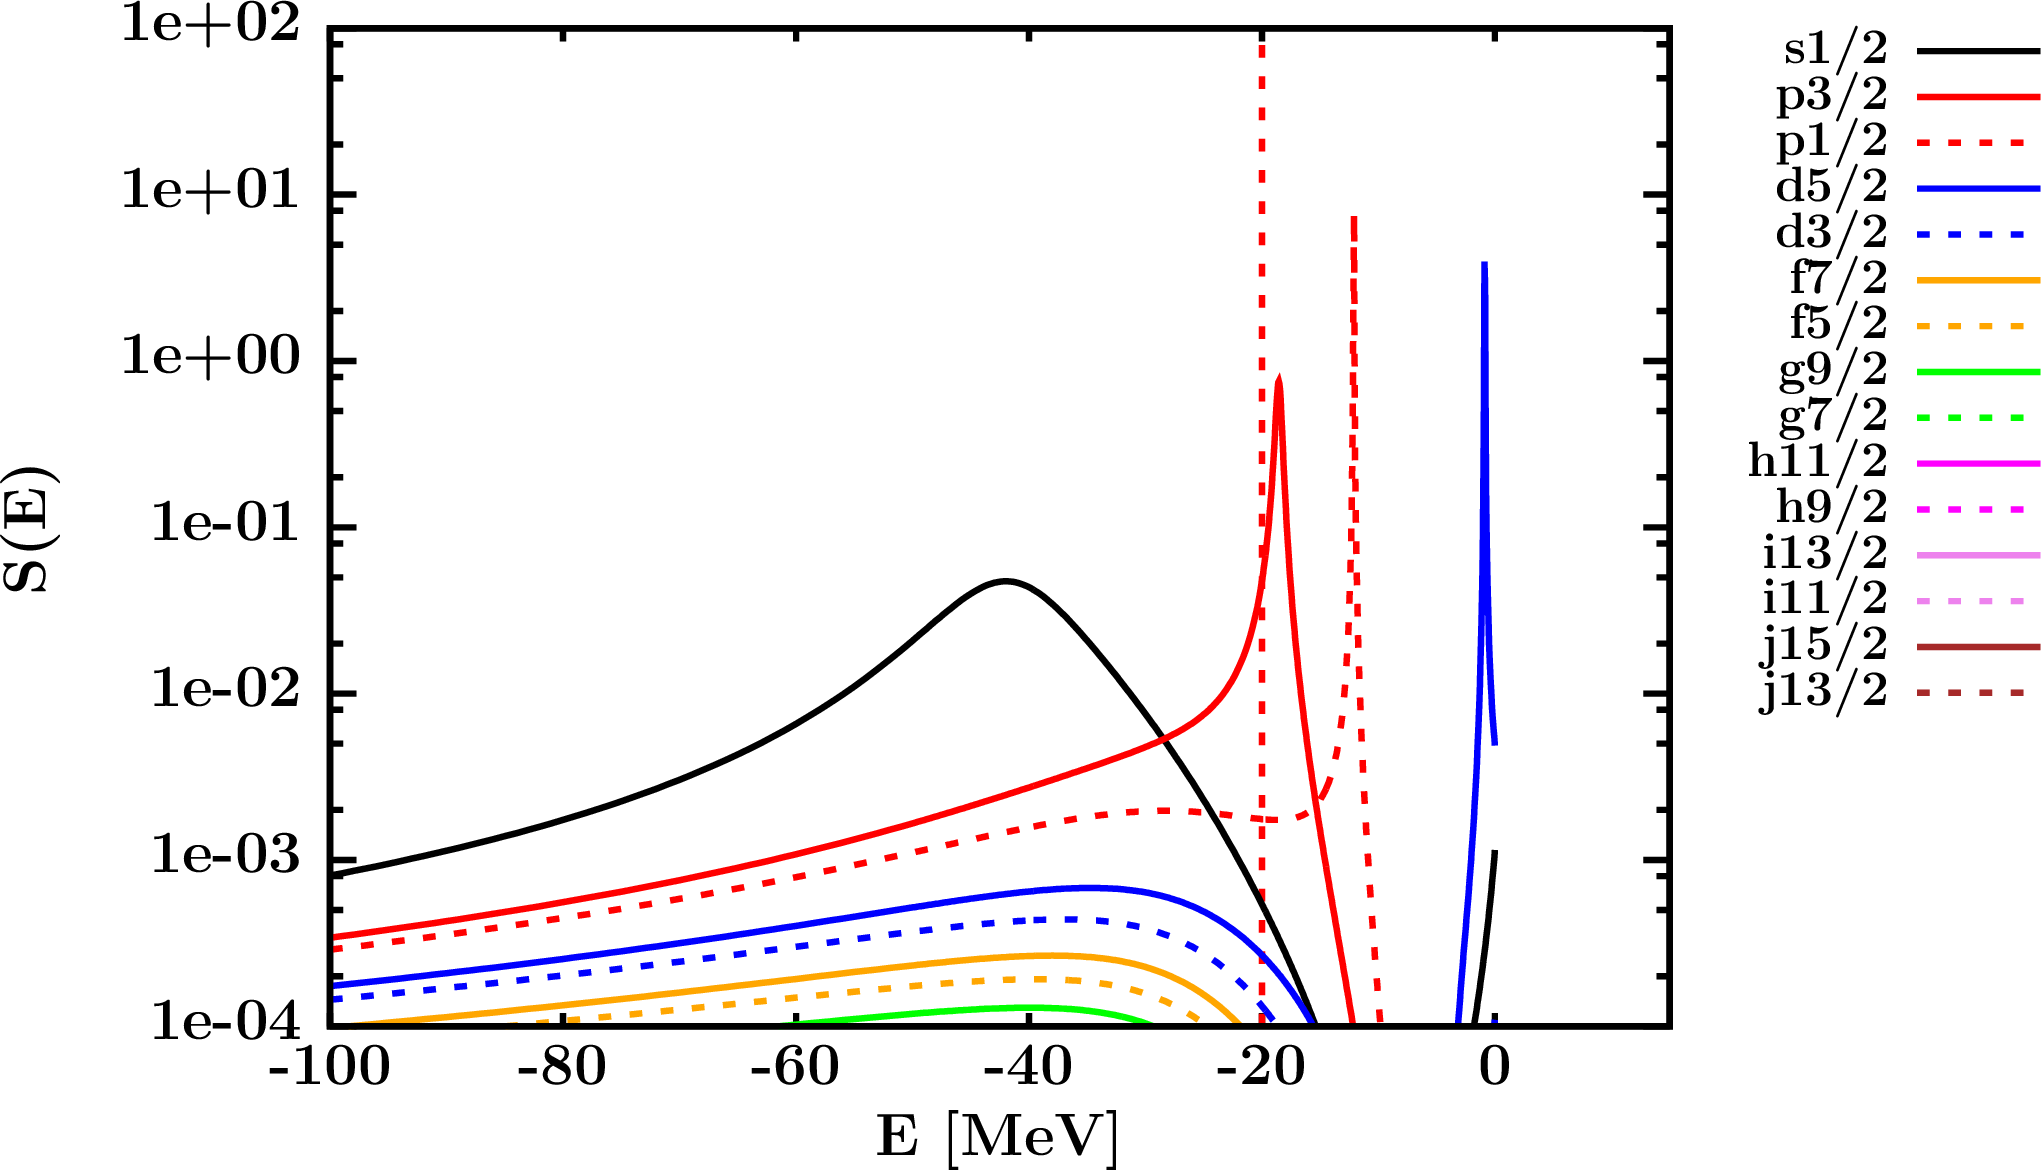
\includegraphics[width = 0.9\textwidth]{figures/o16_protonSpectralFunctions.png}
%\caption{DOM calculation of $^{16}O$ proton spectral functions}
%\label{o16ProtonSpectralFunctions}
%\end{center}
%\end{figure}
%
%
%\begin{figure}
%\begin{center}
%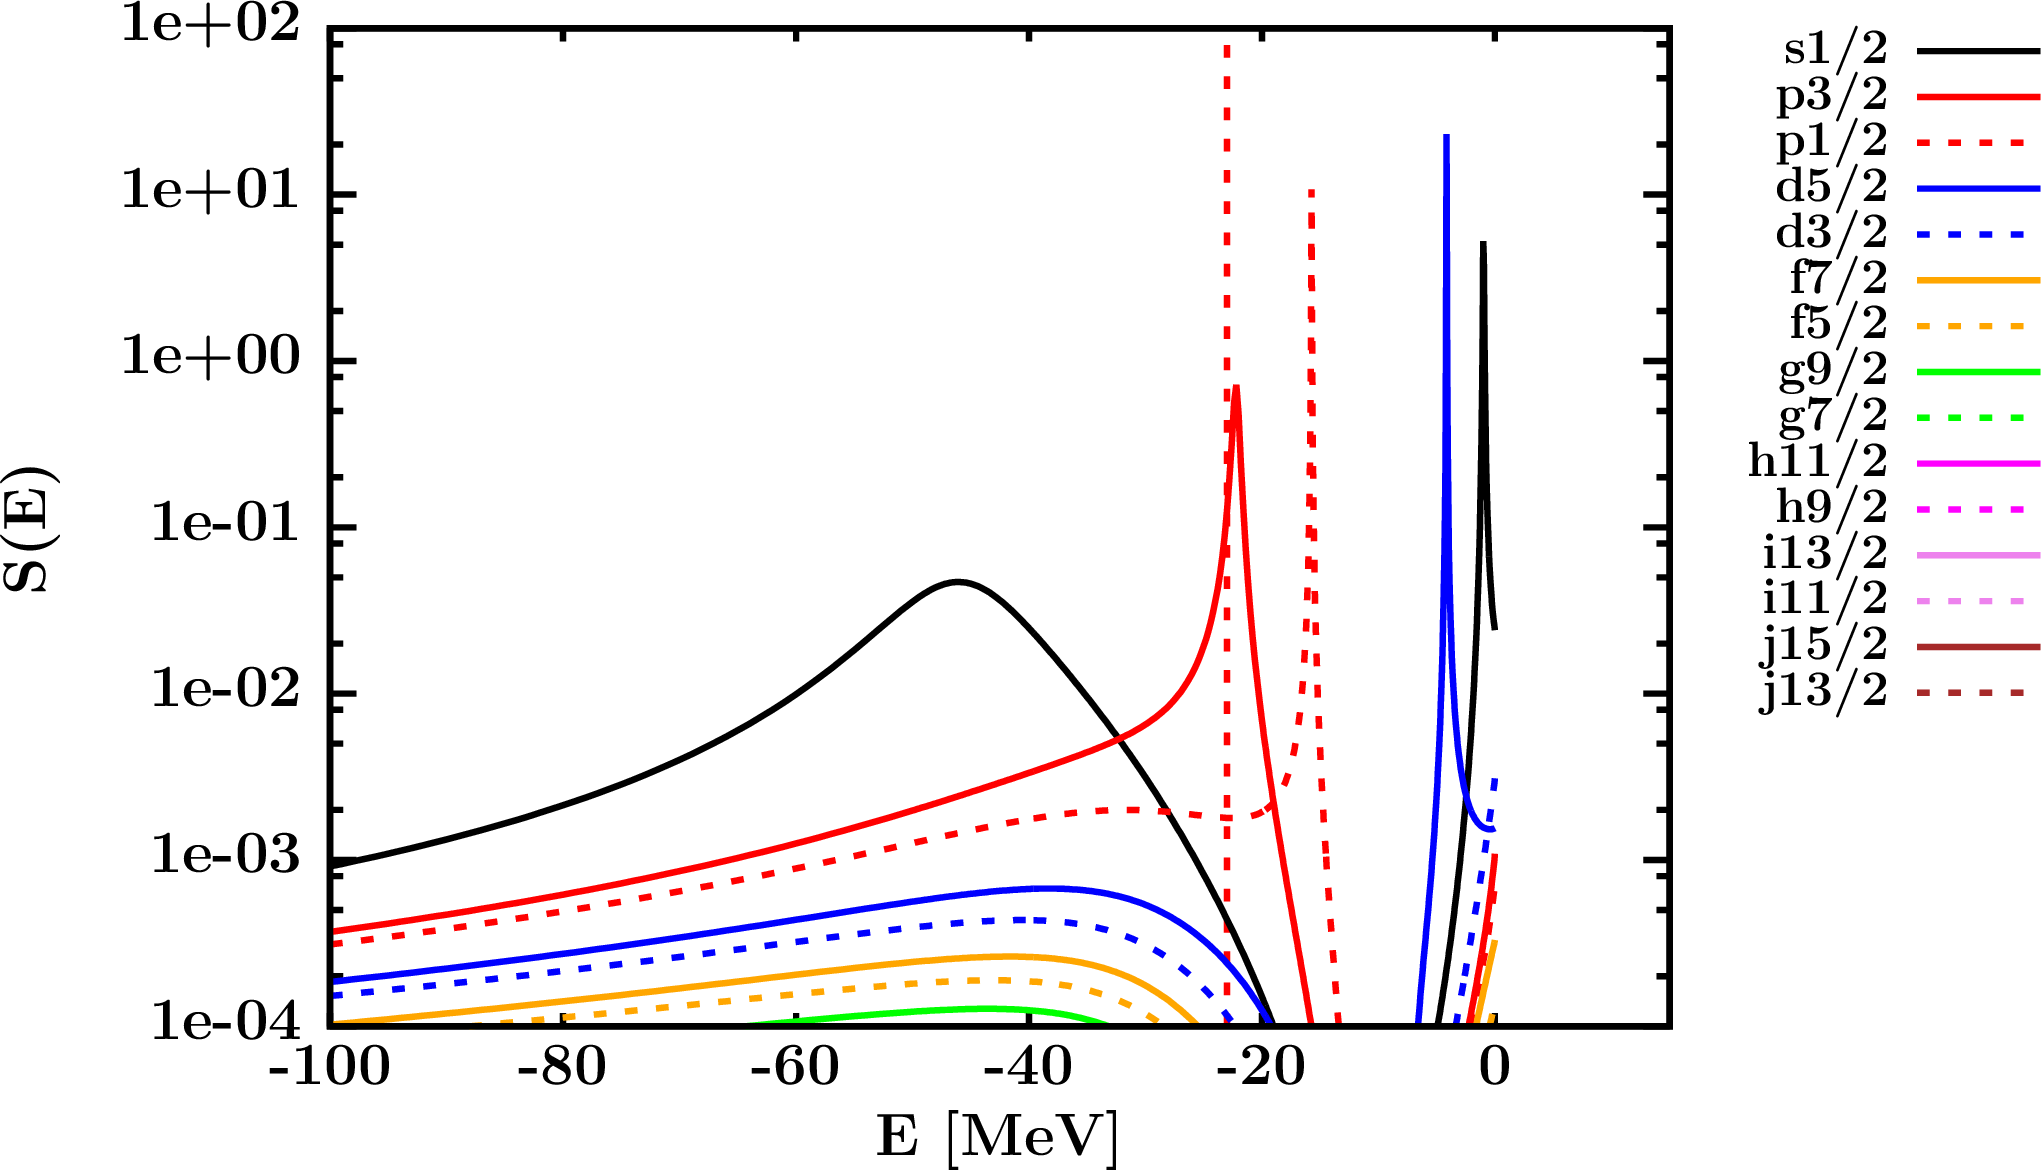
\includegraphics[width = 0.9\textwidth]{figures/o16_neutronSpectralFunctions.png}
%\caption{DOM calculation of $^{16}O$ neutron spectral functions}
%\label{o16NeutronSpectralFunctions}
%\end{center}
%\end{figure}
%
%\begin{figure}
%\begin{center}
%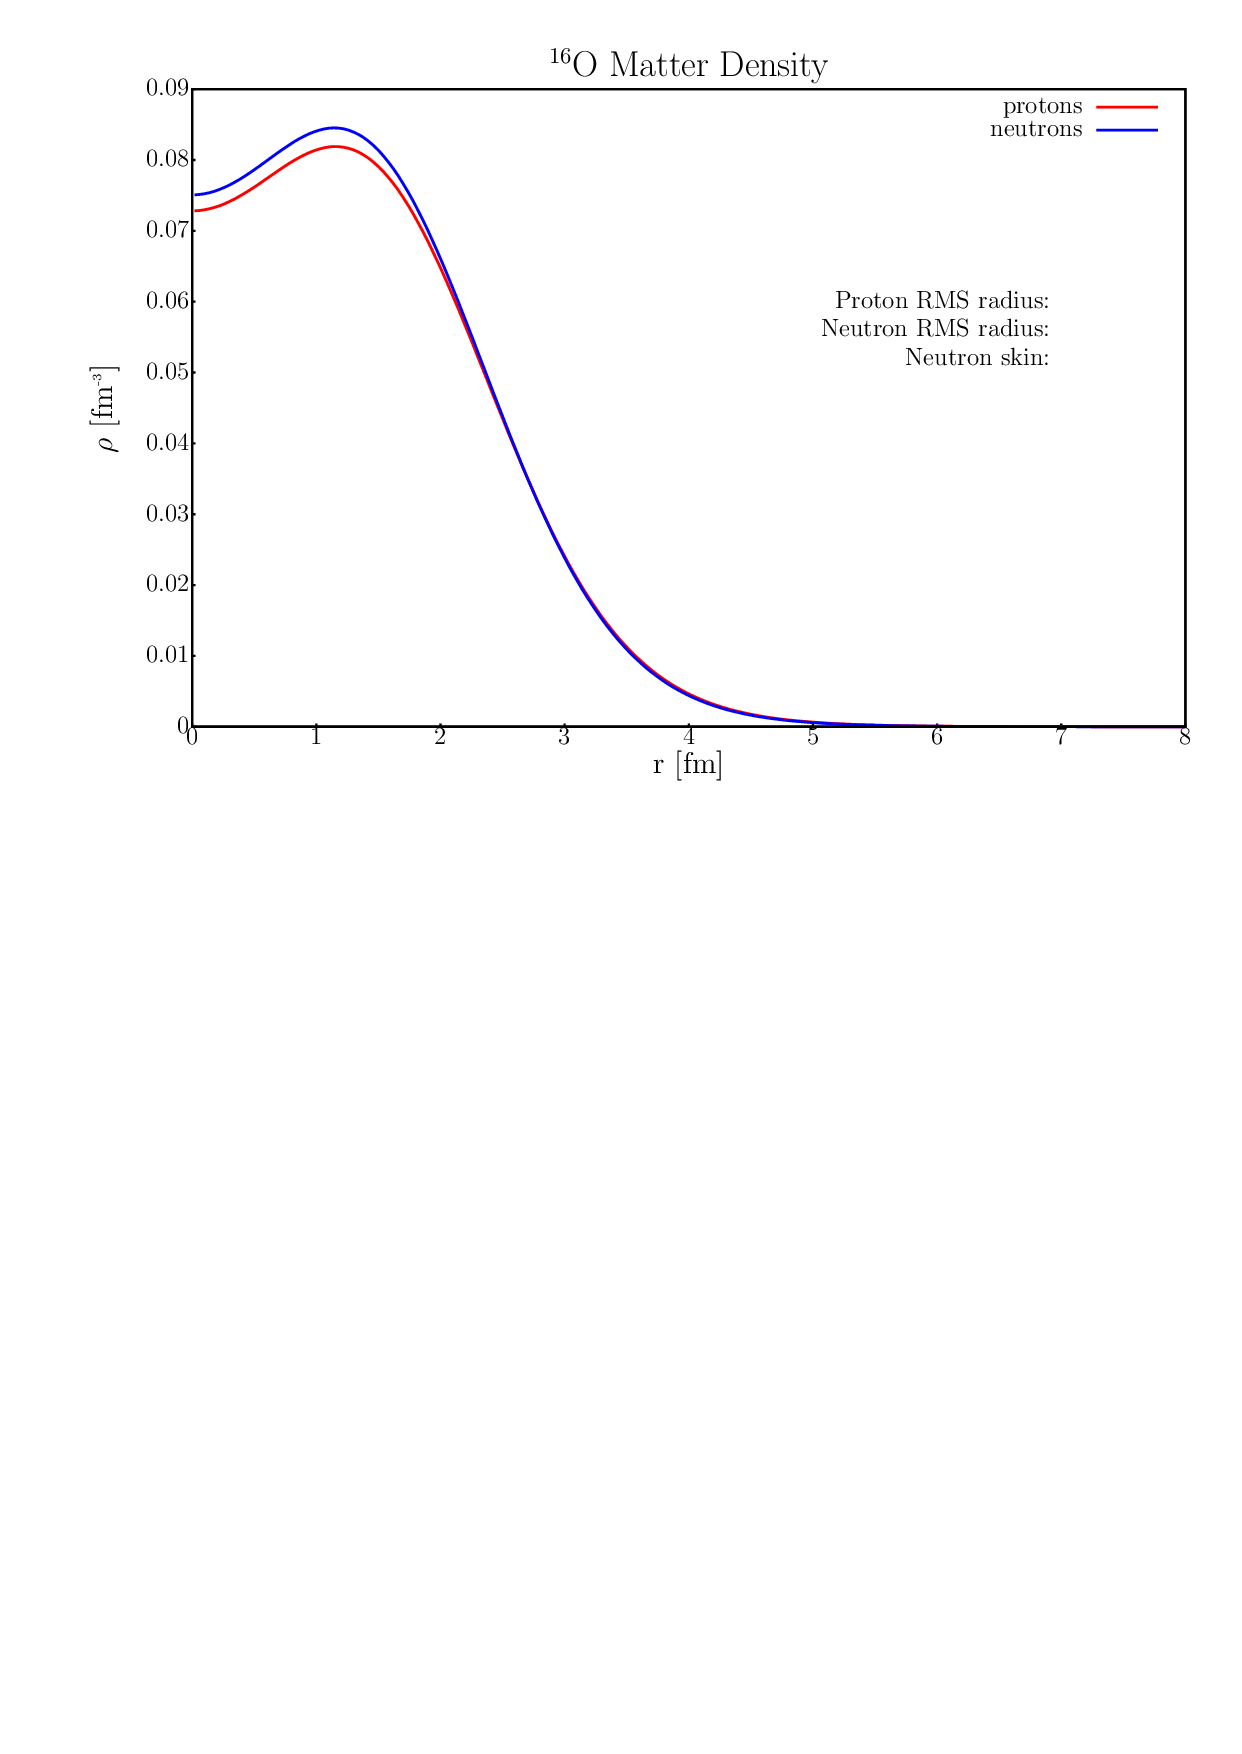
\includegraphics[width = 0.9\textwidth]{figures/o16_matterDensity.png}
%\caption{DOM prediction of $^{16}O$ matter density}
%\label{o16MatterDensity}
%\end{center}
%\end{figure}



\section{Results for \niEightFour}

\section{Results for \snTwelveFour}

\section{Results for \pbEight}
The size of the neutron skin of \pbEight has been identified by numerous studies as highly
correlated with the density-dependence of the symmetry energy, $L$, a critical input for the neutron
star equation-of-state. By employing parity-violating electron scattering to probe the
weak charge distribution in \pbEight, the PREX experiment at Jefferson Laboratory extracted a
\pbEight neutron skin value of 0.33$\pm$0.17 fm. A followup experiment with improved statistics, PREX II,
is slated to run later in 2019, and is expected to constrain the \pbEight neutron skin thickness to
within 0.06 fm. Given the wide range of \pbEight neutron skin thicknesses predicted by relativistic
and non-relativistic mean-field models, an accurate calculation of this quantity is an excellent
test for the validity of the DOM treatment.

%\begin{table}
%  \begin{center}
%    \caption{Calibration beams and the energies generated with the degraders.}\label{CBeams}
%  \begin{tabular}{ccccc}
%    \hline \hline
%    Species & Energy & Target & Thickness & Degraded Energy  \\ 
%            & [MeV/A] & &[mg/cm$^2$] & [MeV/A] \\
%     \hline
%    $p$ & 24.2 &  Au & 20.0 & 24.0   \\
%           &  & Al & 429 & 15.8 \\
%    \hline
%    $d$ & 24.2 &  Au &20.0 & 24.1 \\
%            & & Al & 429 &20.3 \\
%    & &  Al & 858 & 15.8 \\
%            & 12.0 &  Au & 20.0 & 11.9 \\
%    \hline
%    $\alpha$ & 24.0 &  Au & 20.0 & 23.8 \\
%     & & Al & 429 &15.6 \\
%    \hline \hline
%  \end{tabular}
%\end{center}
%\end{table}

\section{General trends}
\subsection{Neutron skins sensitive to shell structure}
- too little data fixing the imaginary surface below. Difficulty in separating the imaginary surface
below and imaginary volume below, especially for lighter nuclei (Ni and lower).
\subsection{Depletion essential for recovering high-momentum content}
\subsection{Overestimation of RMS charge radius due to extra density in distribution tail}
\subsection{Need for covariance analysis}

\afterpage{\clearpage}
